% Copyright (C) 2021 Erwin Müller <erwin@muellerpublic.de>
% Released as open-source under the Apache License, Version 2.0.
%
% ****************************************************************************
% ANL-OpenCL :: Docs
% ****************************************************************************
%
% Copyright (C) 2021 Erwin Müller <erwin@muellerpublic.de>
%
% Licensed under the Apache License, Version 2.0 (the "License");
% you may not use this file except in compliance with the License.
% You may obtain a copy of the License at
%
%      http://www.apache.org/licenses/LICENSE-2.0
%
% Unless required by applicable law or agreed to in writing, software
% distributed under the License is distributed on an "AS IS" BASIS,
% WITHOUT WARRANTIES OR CONDITIONS OF ANY KIND, either express or implied.
% See the License for the specific language governing permissions and
% limitations under the License.
%
% ****************************************************************************
% ANL-OpenCL :: Docs is a derivative work based on Josua Tippetts' C++ library:
% http://accidentalnoise.sourceforge.net/index.html
% ****************************************************************************
%
% Copyright (C) 2011 Joshua Tippetts
%
%   This software is provided 'as-is', without any express or implied
%   warranty.  In no event will the authors be held liable for any damages
%   arising from the use of this software.
%
%   Permission is granted to anyone to use this software for any purpose,
%   including commercial applications, and to alter it and redistribute it
%   freely, subject to the following restrictions:
%
%   1. The origin of this software must not be misrepresented; you must not
%      claim that you wrote the original software. If you use this software
%      in a product, an acknowledgment in the product documentation would be
%      appreciated but is not required.
%   2. Altered source versions must be plainly marked as such, and must not be
%      misrepresented as being the original software.
%   3. This notice may not be removed or altered from any source distribution.
%
%
% ****************************************************************************
% ANL-OpenCL :: Docs bundles and uses the RandomCL library:
% https://github.com/bstatcomp/RandomCL
% ****************************************************************************
%
% BSD 3-Clause License
%
% Copyright (c) 2018, Tadej Ciglarič, Erik Štrumbelj, Rok Češnovar. All rights reserved.
%
% Redistribution and use in source and binary forms, with or without modification, are permitted provided that the following conditions are met:
%
% * Redistributions of source code must retain the above copyright notice, this list of conditions and the following disclaimer.
%
% * Redistributions in binary form must reproduce the above copyright notice, this list of conditions and the following disclaimer in the documentation and/or other materials provided with the distribution.
%
% * Neither the name of the copyright holder nor the names of its contributors may be used to endorse or promote products derived from this software without specific prior written permission.
%
% THIS SOFTWARE IS PROVIDED BY THE COPYRIGHT HOLDERS AND CONTRIBUTORS "AS IS" AND ANY EXPRESS OR IMPLIED WARRANTIES, INCLUDING, BUT NOT LIMITED TO, THE IMPLIED WARRANTIES OF MERCHANTABILITY AND FITNESS FOR A PARTICULAR PURPOSE ARE DISCLAIMED. IN NO EVENT SHALL THE COPYRIGHT HOLDER OR CONTRIBUTORS BE LIABLE FOR ANY DIRECT, INDIRECT, INCIDENTAL, SPECIAL, EXEMPLARY, OR CONSEQUENTIAL DAMAGES (INCLUDING, BUT NOT LIMITED TO, PROCUREMENT OF SUBSTITUTE GOODS OR SERVICES; LOSS OF USE, DATA, OR PROFITS; OR BUSINESS INTERRUPTION) HOWEVER CAUSED AND ON ANY THEORY OF LIABILITY, WHETHER IN CONTRACT, STRICT LIABILITY, OR TORT (INCLUDING NEGLIGENCE OR OTHERWISE) ARISING IN ANY WAY OUT OF THE USE OF THIS SOFTWARE, EVEN IF ADVISED OF THE POSSIBILITY OF SUCH DAMAGE.

\section{App}

\begin{figure}
\centering
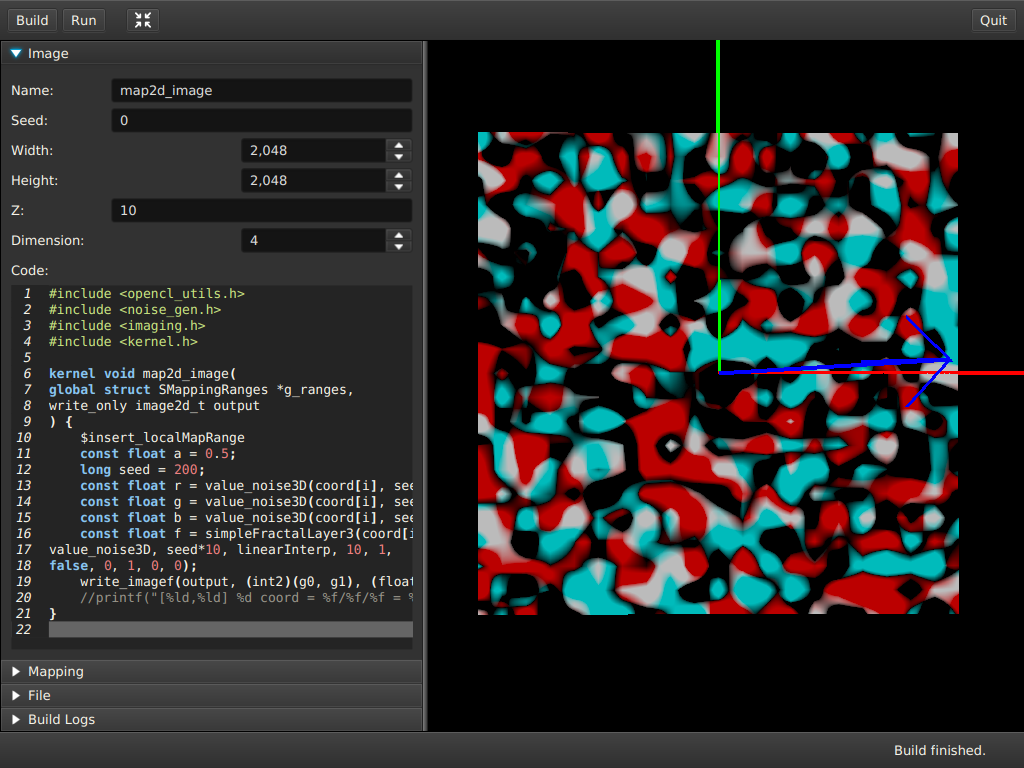
\includegraphics[width=0.4\textwidth]{Screenshot_20211121_152848.png}
\caption{Screenshot of the app version 0.0.2}\label{fig:app_screenshot}
\end{figure}

The bundled app is a graphical user interface to enter the kernel code, build
it and generate a preview of the noise image. It is implemented 
in Java and JMonkeyEngine 3. The goal of the app is to quickly prototype
noise images with kernel code. The goal is not to provide an IDE or an advanced
code editor. The app is divided into two parts. One part is to enter the kernel code and
parameters and other other part is to display the generated images.

\subsection{Toolbar}

\begin{figure}[h]
\centering

\includegraphics[width=0.4\textwidth]{imgs/toolbar-screenshot-0.png}
\caption{Toolbar}\label{fig:toolbar-screenshot-0}
\end{figure}

The toolbar have buttons for the most common functions.

\subsubsection{Build}

\begin{figure}[h]
\centering
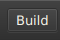
\includegraphics{imgs/toolbar-build-0.png}
\caption{Toolbar Build Button}\label{fig:toolbar-build-0}
\end{figure}

The Build button will build the kernel code and display the generated image
according to the parameters.

\subsubsection{Reset Camera}

\begin{figure}[h]
\centering

\includegraphics{imgs/toolbar-reset-camera-0.png}
\caption{Toolbar Build Button}\label{fig:toolbar-reset-camera-0}
\end{figure}

The Reset Camera button will reset the camera to the default position and zoom.
Key shortcut F10.

\subsubsection{Quit}

\begin{figure}[h]
\centering

\includegraphics{imgs/toolbar-quit-0.png}
\caption{Toolbar Build Button}\label{fig:toolbar-quit-0}
\end{figure}

The Quit button will exit the app. Key shortcut Ctrl-Q.

\label{sec:image}\subsection{Image}

\begin{figure}[h]
\centering
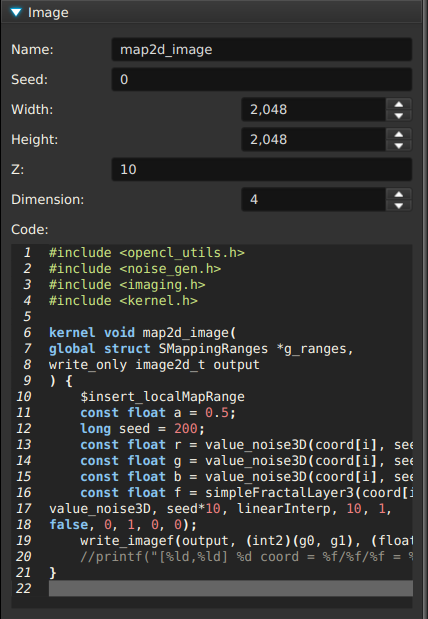
\includegraphics[width=0.4\textwidth]{imgs/main-image-0.png}
\caption{Image}\label{fig:main-image-0}
\end{figure}

The image window have the image parameters and the kernel code.

\subsubsection{Name}

The name of the kernel to build.

\subsubsection{Seed}

The seed number.

\subsubsection{Width}

The width of the image in pixels.

\subsubsection{Height}

The height of the image in pixels.

\subsubsection{Z}

The Z value.

\subsubsection{Dimension}

The count of float numbers of each coordinate. Different noise functions
expect to have the correct dimension of the coordinates available.

\begin{description}
\item[2D] requires dimension of 2 for \texttt{float2};
\item[3D] requires dimension of 4 for \texttt{float3};
\item[4D] requires dimension of 4 for \texttt{float4};
\item[6D] requires dimension of 8 for \texttt{float8};
\end{description}

\label{sec:mapping}\subsection{Mapping}

\begin{figure}[h]
\centering
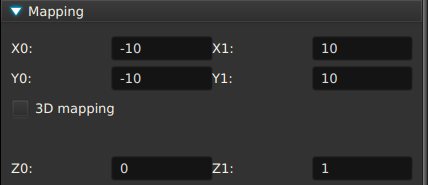
\includegraphics[width=0.4\textwidth]{imgs/main-mapping-0.png}
\caption{Image}\label{fig:main-mapping-0}
\end{figure}

The mapping window have the parameters to map coordinates.

\subsubsection{3D mapping}

If enabled then the mapping is done in 3D and the function \texttt{map3D} must be used.

\subsection{Scene Window}

\begin{figure}[h]
\centering
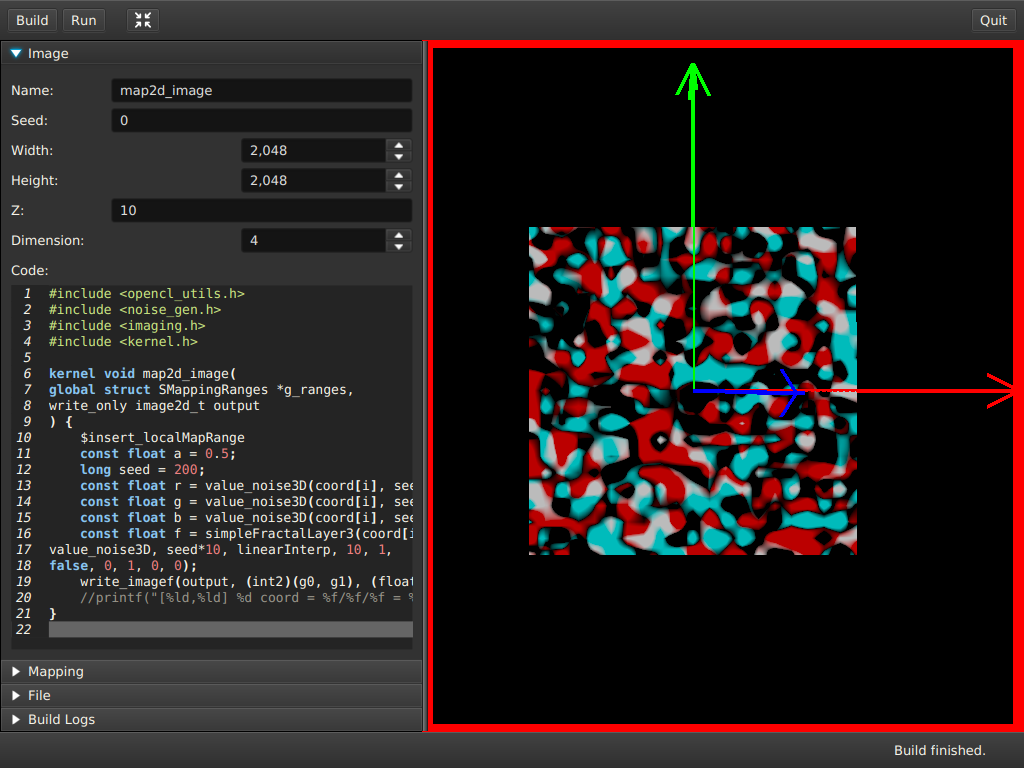
\includegraphics[width=0.4\textwidth]{imgs/main-scene-0.png}
\caption{Image}\label{fig:main-scene-0}
\end{figure}

The scene window shows the generated images. The scene can be moved and zoomed
with the mouse.

\begin{description}
\item[Middle Mouse] moving the scene;
\item[Mouse Wheel] zooming the scene;
\end{description}

